\documentclass[tikz,border=5pt]{standalone}

\usepackage{pgfplots}
\pgfplotsset{compat=1.18}

\begin{document}

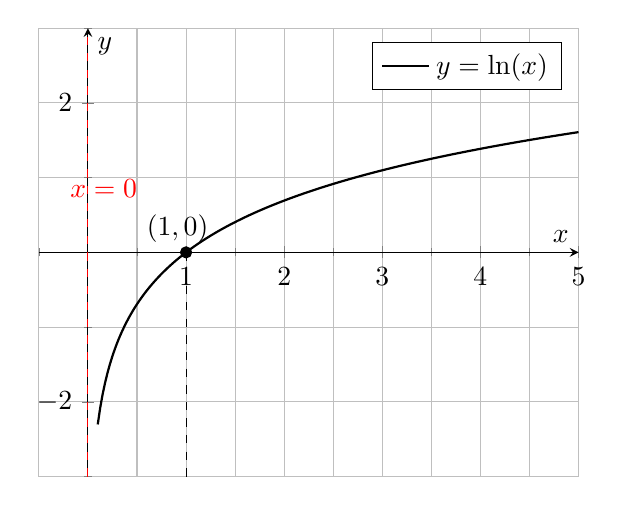
\begin{tikzpicture}
  \begin{axis}[
      axis lines = middle,
      xmin = -0.5, xmax = 5,
      ymin = -3,   ymax = 3,
      samples = 200,
      xlabel = {$x$},
      ylabel = {$y$},
      grid = both,
      minor tick num = 1,
      domain = 0.1:5,
      legend style={at={(0.97,0.97)},anchor=north east},
    ]

    % Plot y = ln(x)
    \addplot[thick, domain=0.1:5] {ln(x)};
    \addlegendentry{$y = \ln(x)$}

    % Vertical asymptote x=0 (dashed, red)
    \addplot[red, dashed] coordinates {(0,-3) (0,3)};

    % Label for asymptote (also red, optional)
    \node[above left, red] at (axis cs:0.6,0.6)
      {$x = 0$};

    % Emphasize the point (1,0)
    \addplot[
      only marks,
      mark=*,
      mark size=2pt
    ] coordinates {(1,0)};

    % Dashed helper lines to the axes
    \addplot[dashed] coordinates {(1,0) (1,-3)};
    \addplot[dashed] coordinates {(0,0) (1,0)};

    % Label the point (moved right/up so it’s off the curve)
    \node[above right] at (axis cs:0.5,0)
      {$(1,0)$};

  \end{axis}
\end{tikzpicture}

\end{document}
